\subsection{Contexto da pesquisa} \label{subsec:contexto}
    Empresas de manufatura e serviços, em geral, trabalham permanentemente com a perspectiva de melhoria contínua. Essa melhoria pode ser obtida por meio da aplicação dos mais diversos métodos e técnicas em várias áreas da produção e etapas do processo, dependendo da necessidade da gerência em resolver determinado problema.
    
    Em um sistema produtivo, o planejamento e programação da produção são etapas importantes no processo de produção, necessitando do uso de técnicas e funções precisas para o melhor desenvolvimento do processo e obtenção de resultados satisfatórios.
    
    O planejamento e a programação são formas de tomada de decisão que são usadas regularmente em indústrias de manufatura e serviços. Ainda, as funções do planejamento e programação em uma empresa dependem de técnicas matemáticas e métodos heurísticos que alocam recursos limitados para as atividades a serem realizadas. Essa alocação de recursos deve ser feita de tal forma que a empresa otimize seus objetivos e alcance suas metas \cite{Pinedo2009}.
    
    Em essência, o planejamento de produção informa quando e quanto produzir (estimativas de capacidade, mão-de-obra, materiais, etc), e a programação da produção informa como produzir (sequenciamento de produção, por exemplo).
    
    Das funções do planejamento e programação da produção, o trabalho explora, para a programação da produção, uma técnica de \textit{scheduling} para problemas modelados usando o princípio de sobreposição de lotes divisíveis (\textit{lot streaming}), para que haja processamento do mesmo lote em paralelo.
    
\subsubsection{Motivação da pesquisa} \label{subsubsec:motivacao}
    Estimar a capacidade de forma precisa pode garantir que o planejamento e programação da produção sejam satisfatórios para o problema apresentado, uma vez que as decisões de capacidade têm um grande impacto em todas as outras questões de planejamento de produção \cite{Hopp2001}. 
    
    Ainda, a importância de uma boa estimativa de capacidade se dá pelo fato de que as decisões tomadas na elaboração de planos de capacidade afetarão vários aspectos diferentes do desempenho, como: os custos, a receita, o capital de giro, a qualidade dos bens ou serviços, a velocidade de resposta à demanda, a confiabilidade da oferta, e a flexibilidade da capacidade \cite{slack2013operations}. 
    
    Não obstante, as técnicas de planejamento de capacidade tem dois objetivos principais: a estimativa e a execução. Se o planejamento da capacidade não é preciso, há então um dos cenários: insuficiência ou excesso de capacidade, e consequentemente seus problemas. Uma capacidade insuficiente leva rapidamente à deterioração do desempenho da entrega, ao aumento dos estoques de \textit{work-in-process} (WIP) e à equipe de manufatura frustrada. Por outro lado, o excesso de capacidade pode ser um gasto desnecessário que pode ser reduzido \cite{Jacobs2011}.
    
    Também, é fato conhecido que em um sistema de produção em lotes, quando o lote de produção é grande, os itens passam maior parte do tempo esperando para serem processados ou esperando o restante do lote para ser então ser transferido à outra estação de trabalho. Ainda, a subdivisão em sublotes menores garante a possibilidade da sobreposição das operações consecutivas a fim de reduzir o tempo total de processamento do lote. De fato, diminuir o tamanho dos lotes possibilita a diminuição do tempo de completude das atividades (\textit{makespan}) \cite{Trietsch1993}. 
    
    Para este trabalho, buscando essa boa estimativa e a diminuição do \textit{makespan}, as técnicas de \textit{lot streaming} foram utilizadas. O \textit{lot streaming} consiste em uma técnica de subdivisão de lotes de produção em sublotes menores, de modo que esses sublotes em operações consecutivas possam ser processados em sobreposição (\textit{overlapping}), isto é, possam ser processados em paralelo.
    
    \textit{Lot streaming} é o processo de dividir um lote em um número de sublotes menores (ou lotes de transferência) para mover os sublotes concluídos de uma máquina (ou estação) para máquinas posteriores para que operações sucessivas possam ser sobrepostas \cite{Ventura2013}.
    
    Quando o \textit{lot streaming} é aplicado, operações (lotes) são divididos em partes menores (sublotes), os quais podem ser processados e transportados individualmente. Se o tamanho dos sublotes forem idênticos para cada operação de um trabalho, os sublotes são chamados consistentes, caso contrário eles são variáveis, os sublotes consistentes são chamados iguais se todos forem do mesmo tamanho. O \textit{lot streaming} é considerado sem intermitência, se todos os sublotes para cada operação tem que ser processado um por um em uma máquina, ou com intermitência, caso contrário \cite{Bozek2017}.
    
    Na Figura~\ref{fig:LSBasic} é ilustrado um exemplo básico do uso das técnicas do \textit{lot streaming}. Há um lote de produção em um sistema de três máquinas com tamanhos de sublotes iguais. Na Figura~\ref{subfig:LS_a}, o tempo de processamento do lote 1 (L1) foi de 3 unidades de tempo na máquina 1 (M1), 3 unidades de tempo na máquina 2 (M2), e 6 unidades de tempo na máquina 3 (M3). Quando o lote não é subdivido, o tempo de completude do lote é de 12 unidades de tempo. Porém, subdividindo o lote L1 em três sublotes de tamanhos iguais (L1, L2 e L3, respectivamente), conforme Figura~\ref{subfig:LS_b}, o tempo de completude diminui, pois ocorreu a sobreposição das operações consecutivas. Portanto, o tempo de completude (\textit{makespan}) desse sistema com a subdivisão é de 8 unidades de tempo.
    
    \begin{figure}[!ht]
    \centering
    \subfigure[\label{subfig:LS_a}]{
    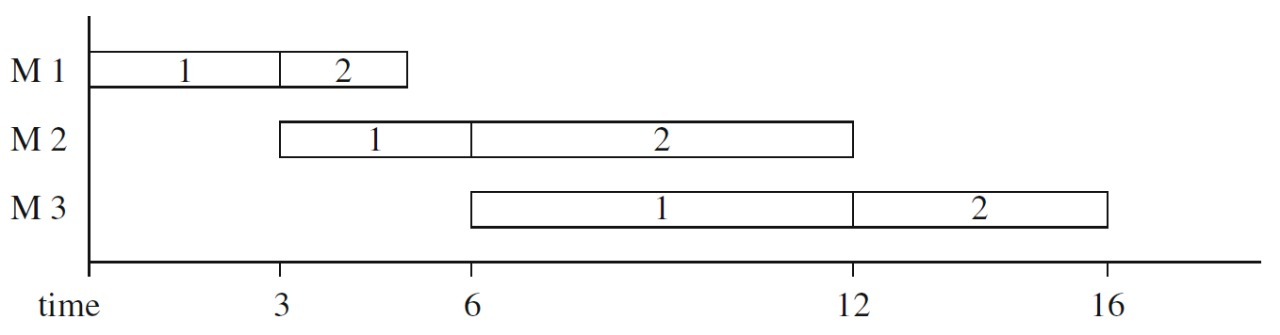
\includegraphics[scale=1]{Introducao/Figuras/Fig_a}
    }
    \subfigure[\label{subfig:LS_b}]{
    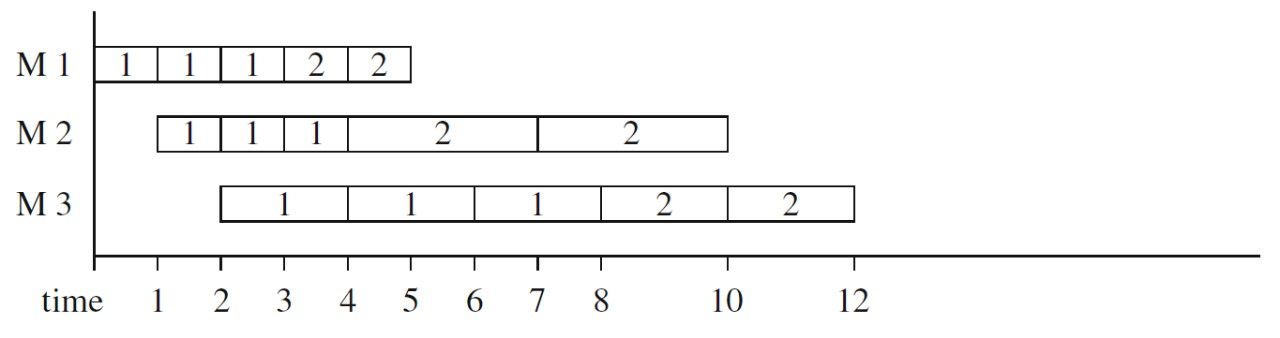
\includegraphics[scale=1]{Introducao/Figuras/Fig_b}
    }
\caption{Exemplo de subdivisão de lotes em um sistema de três máquinas, adaptado de \cite{Ventura2013}.}
\label{fig:LSBasic}
\end{figure}    
    
    O \textit{lot streaming} claramente é capaz de diminuir o tempo total de produção (\textit{makespan}), como mostrado no exemplo básico (Figura~\ref{fig:LSBasic}) uma subdivisão simples já é capaz de gerar uma melhoria de 25\%, diminuindo então o \textit{makespan} consequentemente aumentando a capacidade do sistema.
    
    Reiterando, decisões de capacidade têm um impacto estratégico na competitividade da produção. Uma estratégia de capacidade tem um forte efeito direto nos custos e muitos efeitos indiretos no desempenho, influenciando outros problemas de planejamento e controle, incluindo planejamento agregado, programação, e controle de chão de fábrica \cite{Hopp2001}. Ou seja, boas estimativas de capacidade geram bons resultados na produção. 
    
    
    